% $Header: /home/vedranm/bitbucket/beamer/solutions/generic-talks/generic-ornate-15min-45min.en.tex,v 90e850259b8b 2007/01/28 20:48:30 tantau $

\documentclass{beamer}

% This file is a solution template for:

% - Giving a talk on some subject.
% - The talk is between 15min and 45min long.
% - Style is ornate.



% Copyright 2004 by Till Tantau <tantau@users.sourceforge.net>.
%
% In principle, this file can be redistributed and/or modified under
% the terms of the GNU Public License, version 2.
%
% However, this file is supposed to be a template to be modified
% for your own needs. For this reason, if you use this file as a
% template and not specifically distribute it as part of a another
% package/program, I grant the extra permission to freely copy and
% modify this file as you see fit and even to delete this copyright
% notice.


\mode<presentation>
{
  \usetheme{Warsaw}
  % or ...

  \setbeamercovered{transparent}
  % or whatever (possibly just delete it)
}

      \newtheorem{proposition}[theorem]{Proposition}
      \theoremstyle{definition}
      \newtheorem{game}[theorem]{Game}
      \newtheorem{question}[theorem]{Question}

\usepackage[english]{babel}
% or whatever

\usepackage[latin1]{inputenc}
% or whatever

\usepackage{times}
\usepackage[T1]{fontenc}
% Or whatever. Note that the encoding and the font should match. If T1
% does not look nice, try deleting the line with the fontenc.


\usepackage{marvosym} % For \Smiley
\usepackage{verbatim} % for \verbatiminput

\usepackage{tikz}
\usetikzlibrary{matrix} % for diagrams

\title
{Proximal compact spaces are Corson compact}

\subtitle
{2015 Joint Mathematics Meetings at San Antonio} % (optional)

\author%[Author, Another] % (optional, use only with lots of authors)
{Steven~Clontz~\\http://stevenclontz.com}%\inst{1} \and S.~Another\inst{2}}
% - Use the \inst{?} command only if the authors have different
%   affiliation.

\institute[Auburn University] % (optional, but mostly needed)
{
  %\inst{1}%
  Department of Mathematics and Statistics\\
  Auburn University}
  %\and
  %\inst{2}%
  %Department of Theoretical Philosophy\\
  %University of Elsewhere}
% - Use the \inst command only if there are several affiliations.
% - Keep it simple, no one is interested in your street address.

\date[15-01-11] % (optional)
{January 11, 2015}


% If you have a file called "university-logo-filename.xxx", where xxx
% is a graphic format that can be processed by latex or pdflatex,
% resp., then you can add a logo as follows:

 % \pgfdeclareimage[height=1cm]{university-logo}{auburn_logo.png}
 % \logo{\pgfuseimage{university-logo}}



% Delete this, if you do not want the table of contents to pop up at
% the beginning of each subsection:
%\AtBeginSubsection[]
%{
%  \begin{frame}<beamer>{Outline}
%    \tableofcontents[currentsection,currentsubsection]
%  \end{frame}
%}


% If you wish to uncover everything in a step-wise fashion, uncomment
% the following command:

%\beamerdefaultoverlayspecification{<+->}

% Strategy uparrow shortcuts
\newcommand{\win}{\uparrow}
\newcommand{\prewin}{\underset{\text{pre}}{\uparrow}}
\newcommand{\markwin}{\underset{\text{mark}}{\uparrow}}
\newcommand{\tactwin}{\underset{\text{tact}}{\uparrow}}
\newcommand{\kmarkwin}[1]{\underset{#1\text{-mark}}{\uparrow}}
\newcommand{\ktactwin}[1]{\underset{#1\text{-tact}}{\uparrow}}
\newcommand{\codewin}{\underset{\text{code}}{\uparrow}}
\newcommand{\limitwin}{\underset{\text{limit}}{\uparrow}}
\newcommand{\notprewin}{\underset{\text{pre}}{\not\uparrow}}
\newcommand{\notmarkwin}{\underset{\text{mark}}{\not\uparrow}}
\newcommand{\nottactwin}{\underset{\text{tact}}{\not\uparrow}}
\newcommand{\notkmarkwin}[1]{\underset{#1\text{-mark}}{\not\uparrow}}
\newcommand{\notktactwin}[1]{\underset{#1\text{-tact}}{\not\uparrow}}
\newcommand{\notcodewin}{\underset{\text{code}}{\not\uparrow}}
\newcommand{\notlimitwin}{\underset{\text{limit}}{\not\uparrow}}

\newcommand{\oneptcomp}[1]{#1^*}
\newcommand{\oneptlind}[1]{#1^\dagger}
% \newcommand{\sharp}[1]{#1^{\#}}

\newcommand{\congame}[2]{Con_{O,P}(#1,#2)}
\newcommand{\congamehard}[2]{Con_{O,P}^\star(#1,#2)}
\newcommand{\clusgame}[2]{Clus_{O,P}(#1,#2)}
\newcommand{\clusgamehard}[2]{Clus_{O,P}^\star(#1,#2)}

\newcommand{\lfkpgame}[1]{LF_{K,P}(#1)}
\newcommand{\lfklgame}[1]{LF_{K,L}(#1)}

\newcommand{\pfgame}[1]{PF_{F,C}(#1)}

\newcommand{\mengame}[1]{Men_{C,F}(#1)}
\newcommand{\rothgame}[1]{Cov_{C,S}(#1)}
\newcommand{\altrothgame}[1]{Cov_{P,O}(#1)}

\newcommand{\fillgameS}[1]{Fill^{\cup,\subset}_{C,F}(#1)}
\newcommand{\fillgame}[1]{Fill^{\cup,\subseteq}_{C,F}(#1)}
\newcommand{\fillgameOne}[1]{Fill^{1,\subseteq}_{C,F}(#1)}
\newcommand{\fillgameInt}[1]{Fill^{\cap}_{C,F}(#1)}


\newcommand{\bmGame}[1]{BM_{E,N}(#1)}


\newcommand{\recallgame}[2]{Rec^{#1}_{F,S}(#2)}

\newcommand{\proxgame}[1]{Prox_{D,P}(#1)}
\newcommand{\aproxgame}[1]{aProx_{D,P}(#1)}

\newcommand{\SigmaProdR}[1]{\Sigma\mathbb{R}^{#1}}
\newcommand{\sigmaprodtwo}[1]{\Sigma2^{#1}}

\newcommand{\concat}{{^\frown}}
\newcommand{\rest}{\restriction}

\newcommand{\cl}[1]{\overline{#1}}

\newcommand{\pow}[1]{\mc{P}(#1)}

\newcommand{\<}{\langle}
\renewcommand{\>}{\rangle}

\newcommand{\mc}[1]{\mathcal{#1}}

\newcommand{\po}{\mathbb{P}}
\newcommand{\pok}{\po_\kappa}

\newcommand{\Lim}{\mathrm{Lim}}
\newcommand{\Suc}{\mathrm{Suc}}

\newcommand{\ds}{\displaystyle}

\newcommand{\st}[2]{st\left(#1,#2\right)}


\newcommand{\al}[1]{{#1}^*}
\newcommand{\alcomp}{\wr}

\newcommand{\rank}{\textrm{rank}}
\newcommand{\dom}{\textrm{dom}}

\renewcommand{\mod}{\,\textrm{mod}}

\newcommand{\zip}{\bowtie}
\newcommand{\ran}[1]{\text{range}(#1)}

\newcommand{\cf}[1]{\textrm{cf}(#1)}

\newcommand{\alcompS}[1]{S(#1)}


\newcommand{\scish}{almost-$\sigma$-(relatively compact)}

\usepackage{mathrsfs}
\newcommand{\pl}[1]{\mathscr{#1}}



\newcommand{\term}{\textit}


\newcommand{\bakergame}[1]{{Lim}_{A,B}(#1)}
\newcommand{\bmgame}[1]{{Empty}_{E,N}(#1)}




\begin{document}
\renewcommand{\pause}{}
\newcommand{\vspacing}{\vspace{1em}}
\newcommand{\vpause}{\pause\vspacing}

\begin{frame}
  \titlepage
\end{frame}

\section{Topological Games}

\subsection{Defintion}

\begin{frame}
  A \term{topological game} is a two-player game $G(X)$ of length
  $\omega=\{0,1,2,\dots\}$ defined for certain topological spaces $X$.

  \vpause

  During each round $n$, the first and second player take turns choosing
  certain topological objects from $X$ (e.g. point, open set, open cover, etc.).

  \vpause

  At the ``end'' of the game, a winner is declared by inspecting the sequences
  of choices made throughout the game.

  \vpause

  The study of such games involves finding when a player has a
  \term{winning strategy} which defeats every possible counterattack by
  the opponent.
\end{frame}

\subsection{Example}

\begin{frame}
  \small
  Canonical example: \term{Banach-Mazur Game} (1935) \cite{MR666400}

  \begin{figure}
    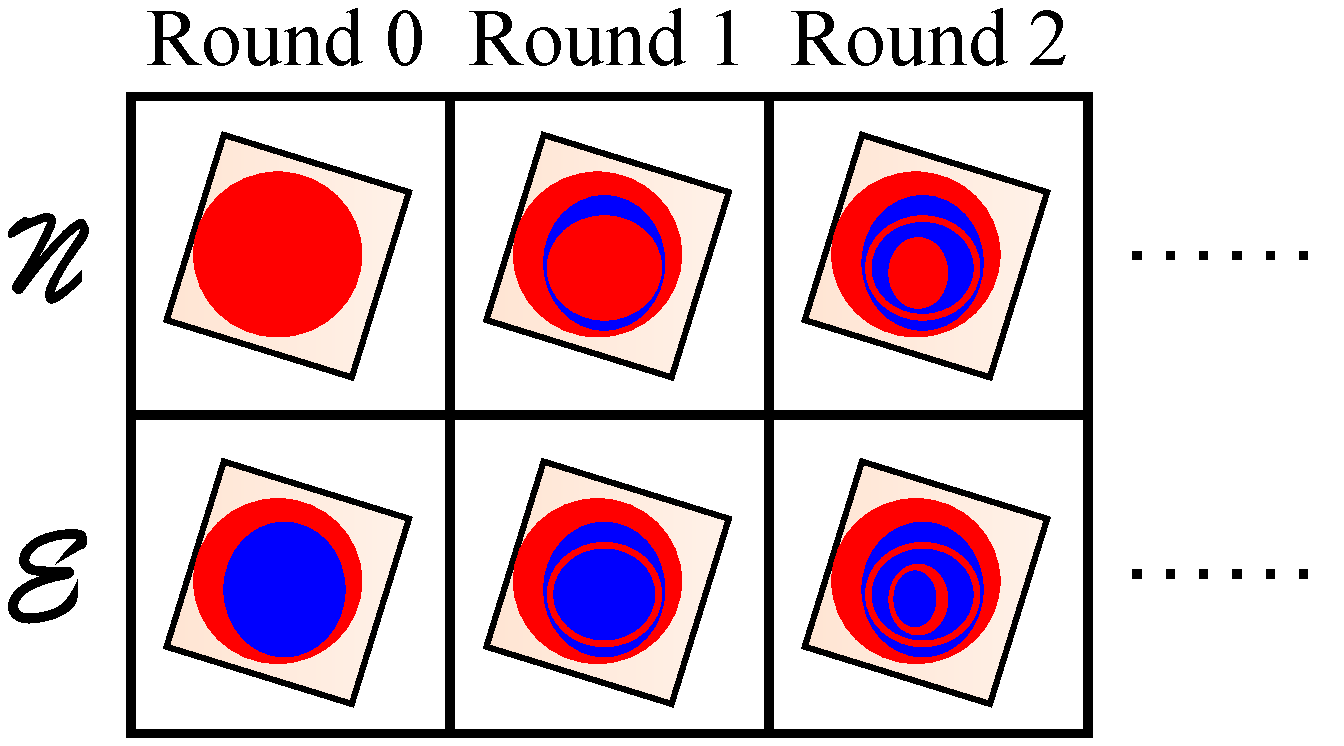
\includegraphics[width=0.6\linewidth]{bmGame.pdf}
  \end{figure}

  \pause

  The first player $\pl N$ wins the game if the intersection of all the chosen
  open sets is nonempty.

  \pause

  \begin{theorem}
    $X$ is Baire if and only if $\pl N$ lacks a winning strategy
    in the Banach Mazur game.
  \end{theorem}

  See Telgarsky's excellent survey on topological games for more
  details: \cite{MR892457}
\end{frame}


\subsection{Proximal Game}

\begin{frame}
  \term{Proximal Game} (2011)
  \cite{MR3239205}

  \vspacing

  \begin{figure}
    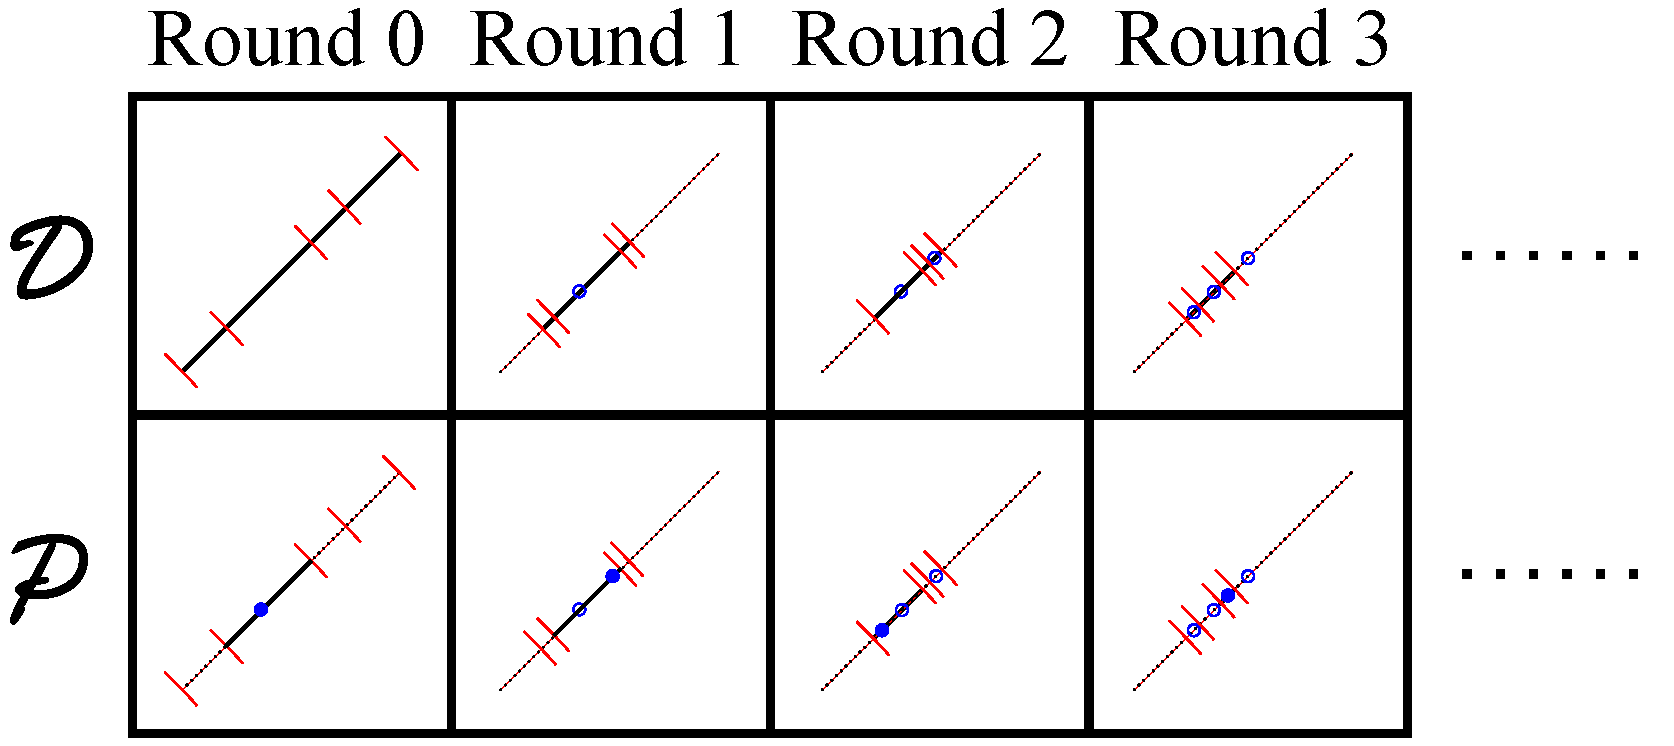
\includegraphics[width=0.8\linewidth]{proximalGame.pdf}
  \end{figure}
  {\tiny for compact $T_1$ $0$-dim spaces}

  \vpause

  The first player $\pl D$ wins the game if the points chosen by the
  second player $\pl P$ converge. If $\pl D$ has a winning
  strategy for this game, call $X$ \term{proximal}.
\end{frame}

\begin{frame}
  Some results related to the Proximal Game due to Jocelyn Bell:

  \begin{proposition}
    If $X$ is metrizable, then $X$ is proximal.
  \end{proposition}

  \begin{theorem}
    If $X$ is proximal, then $X$ is collectionwise normal.
  \end{theorem}

  \begin{theorem}
    $\Sigma$-product and closed subspaces of proximal spaces are proximal.
  \end{theorem}

  \pause

  \begin{corollary}
    The $\Sigma$-product of metrizable spaces is collectionwise normal.
    \cite{MR0461410} \cite{MR716576}
  \end{corollary}
\end{frame}

\section{Main Result}

\subsection{Corson compact}

\begin{frame}
  A \term{Corson compact} space is a space homeomorphic to a compact
  subset of the $\Sigma$-product of real lines.

  \vpause

  Peter Nyikos observed:

  \begin{proposition}
    Every Corson compact space is proximal compact. \cite{nyikosProximalPreprint}
  \end{proposition}

  \pause

  C. and Gruenhage showed in \cite{MR3227201} that any compact proximal
  space must be Corson compact, using another game-theoretic characterization
  of Corson compact due to Gruenhage:
\end{frame}

\subsection{Showing proximal compact implies Corson compact}

\begin{frame}
  \small
  \term{Diagonal Game} (1984) \cite{MR752278}:

  \begin{figure}
    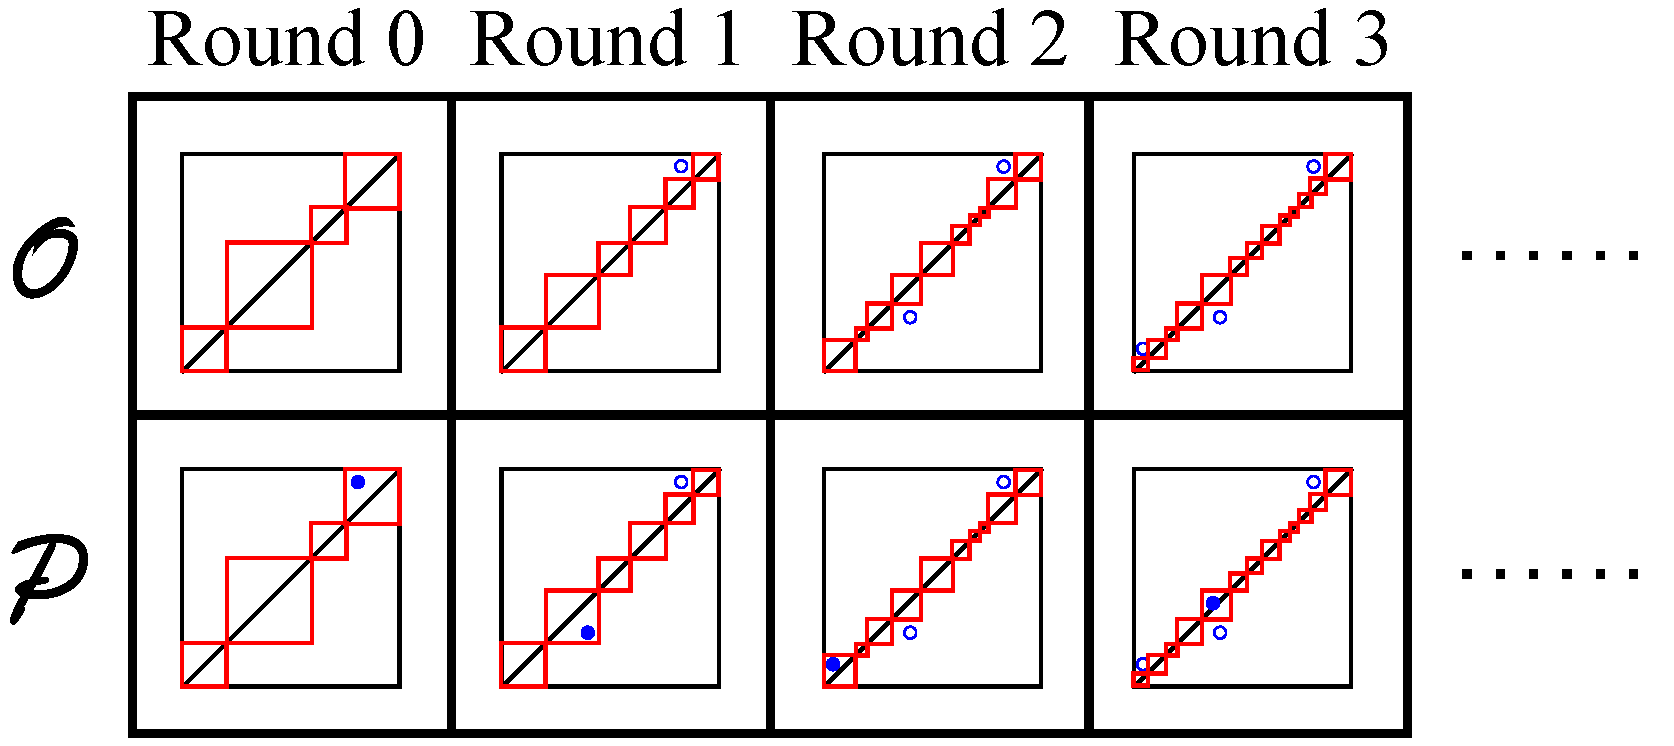
\includegraphics[width=0.7\linewidth]{diagonalGame.pdf}
  \end{figure}
  {\tiny for compact $T_1$ $0$-dim spaces}

  \vpause

  The first player $\pl O$ wins the game if any open set containing the
  diagonal also contains infinitely many of $\pl P$'s chosen points.

  \begin{theorem}
    If $\pl O$ has a winning strategy for the diagonal game
    and $X$ is compact, then $X$ is Corson compact.
  \end{theorem}
\end{frame}

\begin{frame}
  One may use a winning strategy $\sigma$ for $\pl D$ in the proximal game to
  construct a strategy $\tau$ for $\pl O$ in the diagonal game.

  \begin{figure}
    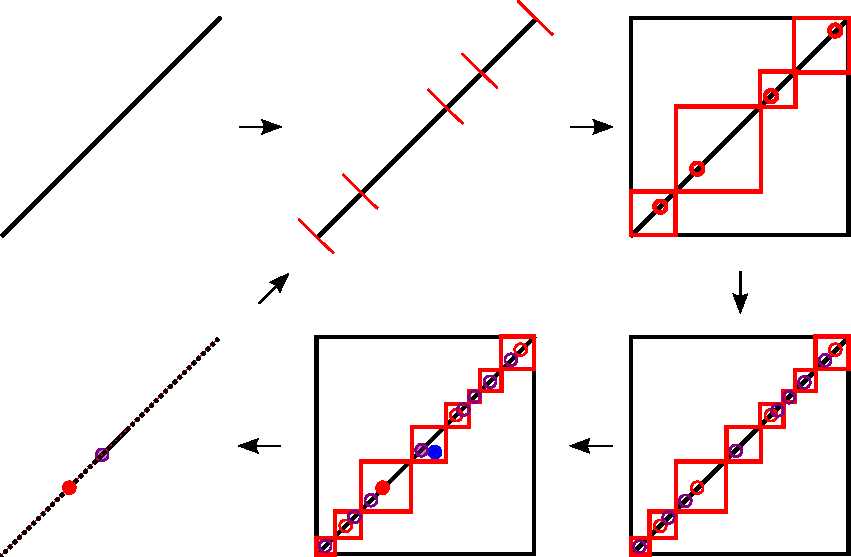
\includegraphics[width=0.7\linewidth]{convertingStrategy.pdf}
  \end{figure}
\end{frame}

\begin{frame}
  In general:
  \[
    \tau(a)
      =
    \bigcup_{s\concat\<i,h_{s,i},j\>\in\max(T(a))}
    \frac{1}{4}\sigma(o_s\concat\<h_{s,i}\>)[h_{s,i,j}]
  \]

  \vspacing

  Using the strategy $\tau$ defined for every proximal compact space,
  $\pl O$ cannot be defeated in the diagonal game, and therefore all
  proximal compacts are Corson compact. \qed
\end{frame}

\section{Questions and References}

\begin{frame}
  Open questions:

  \begin{itemize}
    \item If compactness is dropped, does the proximal game characterize
    all copies of \textit{closed} subspaces of a $\Sigma$-product of reals?
    (Nyikos)
    \item If the winning strategy for the proximal game is \term{Markov}
    (relies on only the latest move and round number) for a compact space,
    does that imply that the space is \term{Eberlein} compact?
    (This holds for the diagonal game.)
  \end{itemize}
\end{frame}


\begin{frame}[allowframebreaks]
  \tiny
  \bibliographystyle{plain}
  \bibliography{../dissertation/bibliography}
\end{frame}

\begin{frame}
  Any questions?
\end{frame}


\end{document}


